\section{Snapshot Mechanism}
\label{sec:snapshot}
An additional challenge that we need to address in the implementation is the excessive log data produced by \intelpt, especially for long running applications. Therefore, we further extended the library to support a live snapshot facility, where the user (or an application using \projecttitle) can analyze the provenance on-the-fly while the program is still running.

For the snapshot facility, the library periodically takes a consistent cut of the CPG. A cut is {\em consistent} if, for any synchronization operation on object $S$ in the trace,  {\em acquire}($S$) operation being in the cut implies that corresponding {\em release}($S$) is also included in the cut~\cite{chandy-lamport}.  To achieve so, we make use of modeling synchronization primitives as {\em acquire} and {\em release} operations (described in $\S$\ref{sec:algorithms}). Each thread invokes the snapshot operation on the latest synchronization event ({\em acquire} or {\em release}) in the recorded trace.


%
\begin{figure}[h]

\centering
      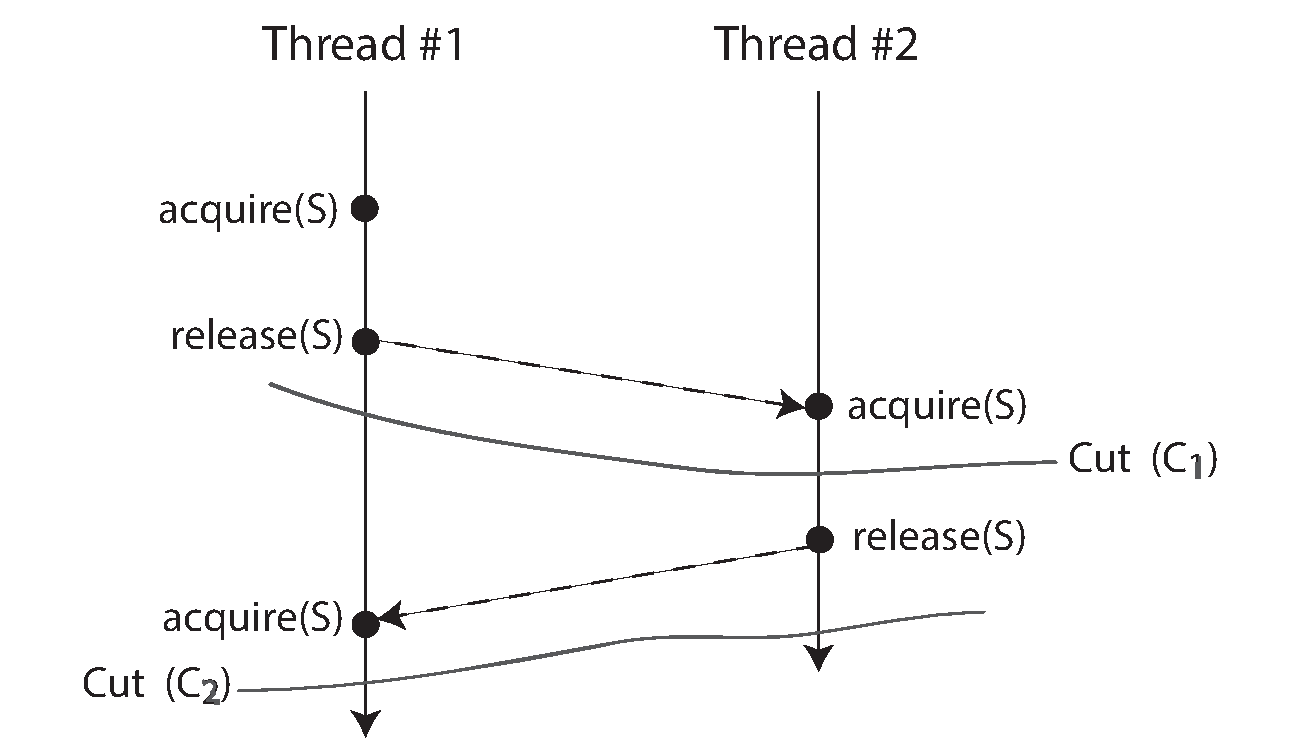
\includegraphics[scale=.3]{figure/snapshot-fig}
  \caption{Consistent cut using acquire and release synchronization primitives.}
   
  \label{fig:snapshot}

\end{figure}



We implemented the snapshot facility using Intel PT interface for {\tt perf},
which provides mechanism for the full trace, and a snapshot mode.
When the full trace is enabled then the kernel overwrites the data that is already processed by
the userspace (indicated by advancing a pointer). This results in gaps in the
trace, if the userspace process is not fast enough in collecting the log data. Whereas, in the snapshot mode, however,
the old data in this ring buffer is constantly overwritten so that an application
can start and stop tracing around a certain event. % By default the snapshot size is 4MB for privileged users. 
The {\tt perf} tool exposes this feature by installing a handler on
signal {\tt SIGUSR2}, which triggers the start of a trace. \projecttitle makes use of the same signal
and forwards it to {\tt perf} to record a  snapshot of the trace for long running programs.
